%% Seção 8: A Evolução Longitudinal da Linguagem e a Trajetória Terapêutica

\chapter{A Evolução Longitudinal da Linguagem e a Trajetória Terapêutica}

\epigrafe{O pensamento e a linguagem são as chaves que abrem todas as portas do conhecimento.}{Lev Vygotsky}

\textbf{8.} A evolução da linguagem ao longo do tempo reflete a trajetória terapêutica do paciente, permitindo medir a eficácia do tratamento e prever possíveis crises ou avanços.

\section{Linguagem como indicador dinâmico}

\textbf{8.1} A linguagem é um indicador dinâmico do estado mental, e sua evolução reflete o progresso ou regressão terapêutica.

\begin{tese}
Se a linguagem reflete o estado mental, então a evolução do discurso ao longo do tempo deve refletir o progresso ou regressão terapêutica.
\end{tese}

\begin{hipotese}[title=Hipótese 8.1.1 (Condicional)]
Se o discurso do paciente se torna mais coerente e articulado ao longo da terapia, então seu estado mental está progredindo positivamente.
\end{hipotese}

\begin{referencia}[title=Referência a Vygotsky]
Lev Vygotsky propõe que o desenvolvimento cognitivo é mediado pela linguagem; assim, a evolução da linguagem indica desenvolvimento mental.
\end{referencia}

\begin{aforismo}
Na progressão da fala, ouve-se o avanço da mente.
\end{aforismo}

\section{Medida da eficácia do tratamento}

\textbf{8.2} A evolução do discurso é uma medida da eficácia do tratamento terapêutico.

\begin{tese}
Se a evolução do discurso reflete a trajetória terapêutica, então a linguagem pode ser usada para medir a eficácia do tratamento.
\end{tese}

\begin{referencia}[title=Referência a Carl Rogers]
A terapia centrada no cliente enfatiza a importância da comunicação autêntica; melhorias na linguagem indicam progresso na congruência interna.
\end{referencia}

\begin{aforismo}
A fala ordenada é o sinal visível de uma mente em recuperação.
\end{aforismo}

\section{Estabilidade e estagnação da linguagem}

\textbf{8.3} A estabilidade ou estagnação da linguagem pode indicar pausas ou obstáculos no progresso terapêutico.

\begin{tese}
Se a estabilidade da linguagem reflete a estabilidade interna, então a interrupção ou estagnação do progresso verbal pode indicar uma pausa no progresso terapêutico.
\end{tese}

\begin{referencia}[title=Referência a Viktor Frankl]
A falta de sentido ou propósito pode levar à estagnação; a linguagem revela essa perda de direção terapêutica.
\end{referencia}

\begin{aforismo}
Quando a fala para de avançar, a mente pode ter encontrado um obstáculo.
\end{aforismo}

\section{Mudanças súbitas na linguagem}

\textbf{8.4} Mudanças súbitas na linguagem podem indicar crises emocionais ou regressões terapêuticas.

\begin{tese}
Se a linguagem evolui junto com o estado mental, então mudanças súbitas no discurso podem indicar crises ou regressões.
\end{tese}

\begin{referencia}[title=Referência a Freud]
Sigmund Freud identificou que crises terapêuticas podem emergir como resistência ou repressão, manifestando-se na linguagem.
\end{referencia}

\begin{aforismo}
A desordem inesperada na fala é o eco de uma mente em turbulência.
\end{aforismo}

\section{Análise longitudinal para previsão}

\textbf{8.5} A análise longitudinal da linguagem permite prever crises ou avanços, ajustando a intervenção terapêutica.

\begin{tese}
Se a linguagem pode ser usada para mapear o progresso terapêutico, então uma análise longitudinal do discurso deve ser aplicada para prever crises ou avanços.
\end{tese}

\begin{referencia}[title=Referência a Aaron Beck]
Na terapia cognitiva, padrões de pensamento negativos são identificados e alterados; a linguagem é fundamental para reconhecer esses padrões e intervir.
\end{referencia}

\begin{aforismo}
A trajetória da fala é um mapa que revela o futuro da mente.
\end{aforismo}

\section{Linguagem como feedback contínuo}

\textbf{8.6} A linguagem como ferramenta de feedback contínuo permite ajustes terapêuticos em tempo real.

\begin{tese}
Se a linguagem fornece feedback sobre o estado interno do paciente, então o terapeuta pode ajustar a intervenção terapêutica de acordo com as mudanças observadas no discurso.
\end{tese}

\begin{referencia}[title=Referência a Milton Erickson]
A terapia breve estratégica utiliza a comunicação como ferramenta central; o terapeuta adapta suas intervenções com base nas respostas linguísticas do paciente.
\end{referencia}

\begin{aforismo}
Na escuta atenta, o terapeuta encontra o caminho para guiar a mente em cura.
\end{aforismo}

%% DIAGRAMA DA SEÇÃO 8
\section*{Diagrama Representativo: Evolução Longitudinal da Linguagem}

\begin{center}
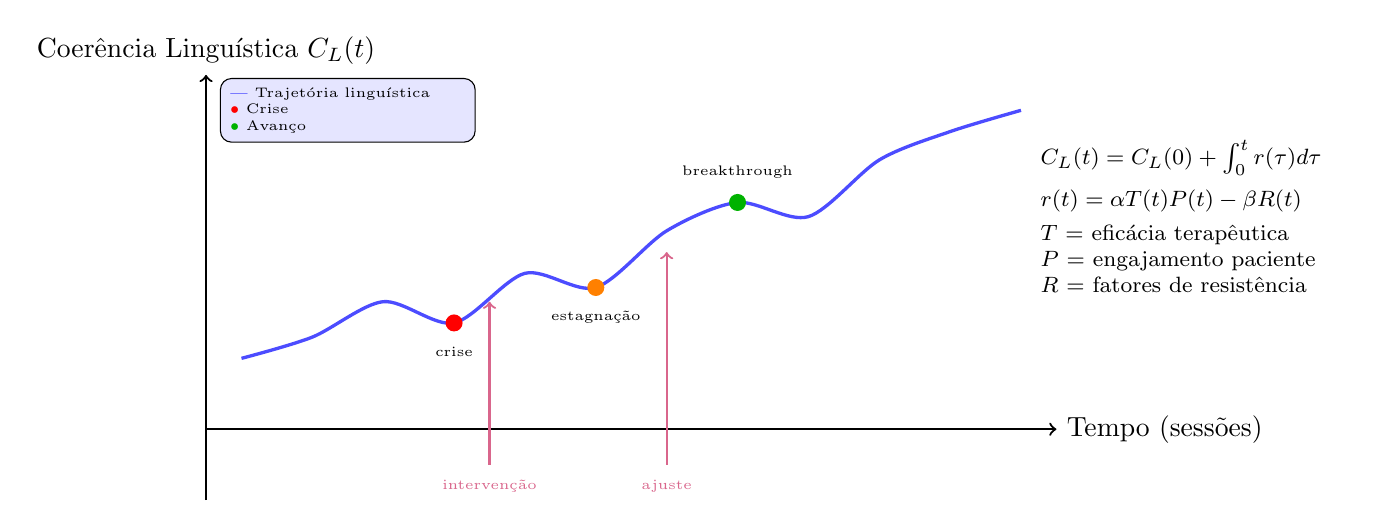
\begin{tikzpicture}[scale=0.9]
    % Eixos
    \draw[thick, ->] (0,0) -- (12,0) node[right] {Tempo (sessões)};
    \draw[thick, ->] (0,-1) -- (0,5) node[above] {Coerência Linguística $C_L(t)$};

    % Curva de evolução
    \draw[very thick, blue!70, smooth] plot coordinates {
        (0.5,1) (1.5,1.3) (2.5,1.8) (3.5,1.5) (4.5,2.2) (5.5,2.0) (6.5,2.8) (7.5,3.2) (8.5,3.0) (9.5,3.8) (10.5,4.2) (11.5,4.5)
    };

    % Marcadores de eventos
    \fill[red] (3.5,1.5) circle (0.12);
    \node[font=\tiny, below] at (3.5,1.3) {crise};

    \fill[orange] (5.5,2.0) circle (0.12);
    \node[font=\tiny, below] at (5.5,1.8) {estagnação};

    \fill[green!70!black] (7.5,3.2) circle (0.12);
    \node[font=\tiny, above] at (7.5,3.4) {breakthrough};

    % Intervenções terapêuticas
    \draw[thick, ->, purple!60] (4,-0.5) -- (4,1.8);
    \node[font=\tiny, purple!60] at (4,-0.8) {intervenção};

    \draw[thick, ->, purple!60] (6.5,-0.5) -- (6.5,2.5);
    \node[font=\tiny, purple!60] at (6.5,-0.8) {ajuste};

    % Fórmula
    \node[font=\footnotesize, text width=4cm, align=left] at (14,3) {
        $C_L(t) = C_L(0) + \int_0^t r(\tau) d\tau$\\[0.5em]
        $r(t) = \alpha T(t) P(t) - \beta R(t)$\\[0.3em]
        \footnotesize $T$ = eficácia terapêutica\\
        \footnotesize $P$ = engajamento paciente\\
        \footnotesize $R$ = fatores de resistência
    };

    % Legenda
    \node[draw, rounded corners, fill=blue!10, font=\tiny, text width=3cm] at (2,4.5) {
        \textcolor{blue}{---} Trajetória linguística\\
        \textcolor{red}{$\bullet$} Crise\\
        \textcolor{green!70!black}{$\bullet$} Avanço
    };
\end{tikzpicture}
\end{center}

\begin{sintese}[title=Síntese Final da Seção 8]
A evolução longitudinal da linguagem é um reflexo direto da trajetória terapêutica do paciente. Conforme Vygotsky, o desenvolvimento cognitivo é mediado pela linguagem, indicando que mudanças no discurso refletem mudanças internas. Carl Rogers enfatiza que a comunicação autêntica é sinal de progresso terapêutico. A estagnação ou regressão na linguagem pode indicar obstáculos ou crises, alinhando-se com as observações de Viktor Frankl sobre perda de sentido e de Freud sobre resistências terapêuticas.

A análise contínua da linguagem permite ao terapeuta não apenas medir a eficácia do tratamento, mas também prever crises ou avanços, ajustando as intervenções conforme necessário. Aaron Beck demonstra que padrões de pensamento negativos podem ser identificados através da linguagem, enquanto Milton Erickson destaca a importância de adaptar a terapia com base no feedback linguístico.
\end{sintese}

\nextpage
